% $Id: taskModel.tex 3909 2013-10-22 06:07:02Z dabhishe $
\vspace{-0.09in}
\section{DREMS Architecture}
\label{sec:task_model}
% This section provides background material and states assumptions for the rest of the paper. 
% in this paper. 
% We also describe the underlying
%system model used for our research.
%\vspace{-0.05in}
%\subsection{\iap\ Architecture}
\iap\ \cite{ISIS_F6_Aerospace:12,6899124,4813} is a distributed system architecture that consists
of one or more computing nodes grouped into a cluster. It is conceptually similar to the recent Fog Computing Architecture \cite{vaquero2014finding}. Distributed applications, composed from cooperating
processes called \textit{actors}, provide services for the end-user.
Actors specialize the notion of OS processes; 
they have persistent identity that allows them to be transparently
migrated between nodes, and they have strict limits on resources that
they can use.  Each actor is constructed from one or more reusable
components~\cite{ISIS_F6_ISORC:13,4813} where each component is
single-threaded.  
% Abhishek, commenting this out.
% Recently, this architecture has been extended to create  applications for smart grid \cite{4813}. 

% \vspace{-0.05in}
% \subsection{The Linux Scheduler}
% \label{sec:linuxScheduler}
% The \iap\ OS scheduler builts upon the standard Linux scheduler
% (kernel version: 3.2.7).  The scheduler is responsible for allocating
% CPU resource(s) to all currently running computational entities.
% Schedulers are implemented in the Linux kernel through \emph{scheduler
%   classes}.  The two important scheduler classes are CFS (Completely Fair
% Scheduler) and the RT (Real Time) scheduler~\cite{mauerer2008}.
% The CFS scheduler attempts to allocate CPU time between processes
% fairly, while the RT scheduler selects processes based on their priority. 

% Tasks eligible for scheduling are maintained in a structure called the
% \emph{runqueue}. Each CPU core has its own runqueue. However
% the runqueue is not necessarily just a queue: it consists of a 
% %-- it is a container using a data structure that contains 
% a bit array,  with one bit for each priority level and a list containing the 
% tasks ready to be scheduled at that level.
% The bit at a level is set to one when there are tasks at that level.
% A 0 value indicates an empty queue at that level. In a multi core
% system, this structure is replicated per CPU. In a fully preemptive
% mode, the scheduling decision is made by  evaluating which task should be
% executed next on a CPU when an interrupt handler exits, when a 
% system call returns, or when the scheduler function is
% explicitly invoked to preempt the current process.

%\begin{figure}[t]
%\centering
%\includegraphics[width=0.45\textwidth]{runqueue}
%\caption{Scheduler Runqueues}
%\label{fig:runqueue}
%\end{figure}

\iffalse
Next sections describe the \iap\ Scheduler features and their main
algorithms. This scheduler was implemented by changing the behavior of
the linux scheduler described in this subsection.  
\fi
\vspace{-0.05in}
%\subsection{Spatial and Temporal Partitioning}
%\label{sec:tasks}

\iffalse
While most tasks\footnote{We use the term threads and tasks
  interchangeably in this paper.} perform application functions,
some tasks are used for system management and mission-critical functions.  
Thus, we group these tasks into different criticality levels: (a) 
\emph{Critical} tasks are those tasks which are required
for system and mission management; (b)
\emph{Application} tasks perform mission-specific, non-critical work; 
(c)
%\emph{System Management}[kernel] tasks provide the interfaces to the
%kernel resources and can be configured to have a fixed percentage of
%CPU time reserved for these tasks; and finally (d)
 \emph{Best Effort}
tasks are those low priority tasks that are scheduled only when there
are no runnable tasks from the previous two categories.
\fi 
\begin{figure}[t]
\centering
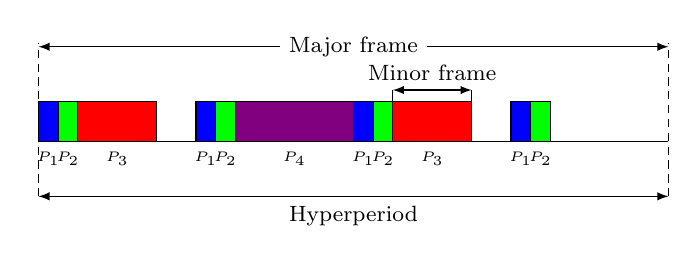
\begin{tikzpicture}[x=1cm,y=1cm, 
every label/.style={font=\tiny},
p1/.style={shape=rectangle,draw,fill=blue, align=center,font=\tiny,minimum height=5mm,minimum width=2.5mm},
p2/.style={shape=rectangle,draw,fill=green,align=center,font=\tiny,minimum height=5mm,minimum width=2.5mm},
p3/.style={shape=rectangle,draw,fill=red,  align=center,font=\tiny,minimum height=5mm,minimum width=10mm},
p4/.style={shape=rectangle,draw,fill=red!50!blue,align=center,font=\tiny,minimum height=5mm,minimum width=15mm},
]
\def\pdist{0.25}\def\hpy{-.95}\def\MF{.95}\def\mfh{.4}\def\mfbeg{17.5*\pdist}\def\mfend{21.5*\pdist}\def\labelpos{270}
\node[p1](P11) at (   0*\pdist,0) [label=\labelpos:$P_1$]{}; \node[p2](P21) at ( 1*\pdist,0) [label=\labelpos:$P_2$] {};
\node[p3](P31) at ( 3.5*\pdist,0) [label=\labelpos:$P_3$]{}; 
\node[p1](P12) at (   8*\pdist,0) [label=\labelpos:$P_1$]{}; \node[p2](P22) at ( 9*\pdist,0) [label=\labelpos:$P_2$] {};
\node[p4](P41) at (12.5*\pdist,0) [label=\labelpos:$P_4$]{}; 
\node[p1](P13) at (  16*\pdist,0) [label=\labelpos:$P_1$]{}; \node[p2](P23) at (17*\pdist,0) [label=\labelpos:$P_2$] {};
\node[p3](P32) at (19.5*\pdist,0) [label=\labelpos:$P_3$]{};
\node[p1](P14) at (  24*\pdist,0) [label=\labelpos:$P_1$]{}; \node[p2](P24) at (25*\pdist,0) [label=\labelpos:$P_2$] {};
\draw[densely dashed,-] (-0.5*\pdist,\hpy) -- (-0.5*\pdist,1); \draw[densely dashed,-] (31.5*\pdist,\hpy) -- (31.5*\pdist,1);
\draw[-] (-0.5*\pdist,-.25) -- (31.5*\pdist,-.25);
\draw[latex-latex] (-0.5*\pdist,\hpy) -- (31.5*\pdist,\hpy) node [below,align=center,midway,font=\footnotesize] {Hyperperiod};
\draw[latex-latex] (-0.5*\pdist,\MF) -- node[sloped,fill=white,font=\footnotesize]{Major frame} (31.5*\pdist,\MF);
%
\draw[-] (\mfbeg,0) -- (\mfbeg,\mfh); \draw[-] (\mfend,0) -- (\mfend,\mfh);
\draw[latex-latex] (\mfbeg,\mfh) -- (\mfend,\mfh) node [above,align=center,midway,font=\footnotesize] {Minor frame};
\end{tikzpicture}%

\caption{A Major Frame. The four partitions (period,duration) in this frame are $P_1$ (2s, 0.25s), $P_2$ (2s, 0.25s), $P_3$ (4s, 1s), and $P_4$ (8s, 1.5s). }
%where the first number is the period and the second number is the duration of the partition.}
\label{fig:validschedule}
\vspace{-0.2in}
\end{figure}

%The length of the repeating frame is also known as the \emph{major frame}.  

%Given a valid schedule as input, the
%scheduler guarantees that actors in separate temporal partitions
%cannot interfere with each other's CPU resource usage.  

%
%
%. For the RT scheduler it is an array combined with bits
%indicating priority. Tasks are added  to the runqueue when they are in ready state and are removed from the runqueue when they are waiting for either a reseource or are sleeping for some time. 
%
%
%
% and removed from the runqueue as they become ready or 
%
%
%The runqueues do not necessarily contain all the
%existing tasks in the system - only those which are eligible for
%scheduling. One example for tasks which are not in any of the queues
%are inactive tasks. When a task becomes inactive it is removed from
%the runqueues (\texttt{dequeue\_task}) and a timer is started. When the
%timer expires, the task is added back to the runqueue
%(\texttt{enqueue\_task}). This dequeuing and enqueing happens each
%time a task changes its state from ready to another state.
%
%When SMP (Symmetric Multiprocessing) is enabled, each CPU manages its own runqueue. Tasks are
%occasionally migrated between CPUs based on a balancing algorithm. The
%RT scheduler runqueue consists of a bitmap and a linked list for each
%priority level. The bitmap contains "1" if the given list contains any
%element - this allows the scheduler to jump to the highest priority 
%ready task in constant time. When a task is added to the list the
%bitmap is updated and the task is added to the linked list belonging
%to the given level. The same steps happen for task removal or a
%change in a task's priority. During a scheduling decision, the
%core scheduler goes through the scheduler classes in their priority
%order and calls the \texttt{pick\_next\_task} function. If it returns with a task, the task will get prioritized. 
%If no task is ready to run, the idle task is scheduled. A 
%scheduling decision happens in one of the following situations:
%
%\begin {itemize}
%\item [A)] When an interrupt handler exits (including the interrupt invoked
%  by the periodic tick timer).
%\item [B)] When a system call returns.
%\item [C)] When the scheduler is invoked explicitly by the current running
%  task.
%\end {itemize}

% TODO:  I presume this has yet to be done?
%{\bf describe the preemption-RT patch}

